\documentclass{beamer}

\mode<presentation>
{
  \usetheme{Antibes}
  \setbeamercovered{transparent}
}

\usepackage[english]{babel}
\usepackage[latin1]{inputenc}
\usepackage{times}
\usepackage[T1]{fontenc} 
% Or whatever. Note that the encoding and the font should match. If T1
% does not look nice, try deleting the line with the fontenc.
\usepackage{amsmath}

\newcommand{\linespace}{\vskip 0.25cm}

\definecolor{MyForestGreen}{rgb}{0,0.7,0} 
\newcommand{\mynotes}[1]{}

% The text in square brackets is the short version of your title and will be used in the
% header/footer depending on your theme.
\title[Interoperability]{Interoperability in Programming Languages}

% Sub-titles are optional - uncomment and edit the next line if you want one.
% \subtitle{Why does sub-tree crossover work?} 

% The text in square brackets is the short version of your name(s) and will be used in the
% header/footer depending on your theme.
\author[Malone]{Todd Owen Malone}

% The text in square brackets is the short version of your institution and will be used in the
% header/footer depending on your theme.
\institute[U of Minn, Morris]
{
  Division of Science and Mathematics \\
  University of Minnesota, Morris \\
  Morris, Minnesota, USA
}

% The text in square brackets is the short version of the date if you need that.
\date[April '14, Senior Sem] % (optional)
{28 April 2014 \\ Senior Seminar}

% Delete this, if you do not want the table of contents to pop up at
% the beginning of each subsection:
\AtBeginSection[]
{
  \begin{frame}<beamer>
    \frametitle{Outline}
    \tableofcontents[currentsection, hideothersubsections]
  \end{frame}
}

\begin{document}

\begin{frame}
  \titlepage
\end{frame}

% For a 20-25 minute senior seminar talk you probably want something like:
% - Two or three major sections (other than the summary).
% - At *most* three subsections per section.
% - Talk about 30s to 2min per frame. So there should probably be between
%   15 and 30 frames, all told.
% Slide notes will be comment under each frame end, or under each column where appropriate.

\section*{Interoperability}

\subsection*{Introduction to Interop}

\begin{frame}
  \frametitle{What is Interop?}
  
  \begin{columns}
  \begin{column}{0.6\textwidth}
  \begin{itemize}
  	\item Interoperability or Interop
  	\item The ability for a system to use parts from another system
	\item In programming languages: The ability of a language to call on code from another language
  \end{itemize}
  \end{column}
%mainly, a program running in one language has the ability to call on aspects of another program, written in a different language  
  
  \begin{column}{0.4\textwidth}
   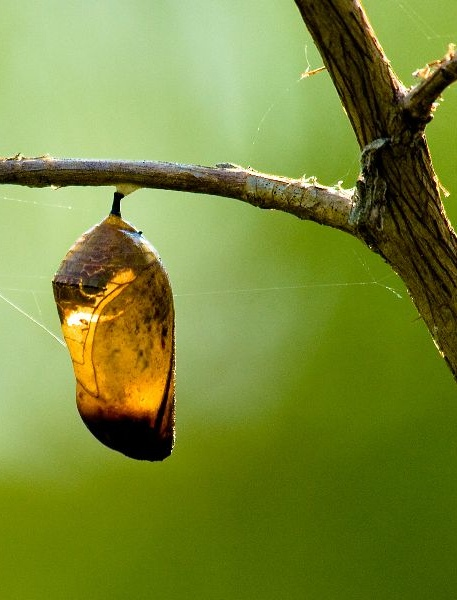
\includegraphics[width=0.95\textwidth]{graphics/Empty_cocoon_crop_by_Bluedrakon_from_Flickr.jpg}
       \\
    \only{\tiny{Bluedrakon \\ \url{http://tr.im/pWUi} }}
  \end{column}
  \end{columns}
\end{frame}

\begin{frame}
  \frametitle{Why is Interop Important?}
%These generally fall under to main categories: Dev time, or effort; and the purpose of different languages.
  
  \begin{columns}[t]
  \begin{column}{0.5\textwidth}
  Developer time and effort
  \begin{itemize}
	\item Existing and working code is easier to use as-is.
  	\item Third-party systems: source code is unavailable
	\item Legacy systems: extensive or little-understood code base.
  \end{itemize}
  \end{column}  


%(consider splitting this into a new slide)
  \begin{column}{0.5\textwidth}
  Language Purpose:
  \begin{itemize}
  	\item Low-level memory access (C)
  	\item Parallel or distributed systems (Erlang, Clojure)
  	\item Statistics (R)
  \end{itemize}
  \end{column}
  \end{columns}
  
\end{frame}

\subsection*{Outline}

\begin{frame}
  \frametitle{Outline}
  \tableofcontents[hideallsubsections]
\end{frame}
%I'll be talking about two particular tools used for enabling interoperability,
%as well as two particular concepts central to interop in programming languages

\section[Interop Tools]{Tools used in achieving interoperability}

\subsection{Virtual Machines}

\begin{frame}
  \frametitle{Virtual Machines}
  
  %add graphic: CLR VM
  \begin{columns}
  \begin{column}{0.6\textwidth}
  \begin{itemize}
	\item Virtual Machines (VMs) are a runtime environment for a program
	\item High-level languages compile to an intermediate language
	\item Intermediate language: Java bytecode or Common Intermediate Language
  \end{itemize}
  \end{column}
  
  \begin{column}{0.5\textwidth}
  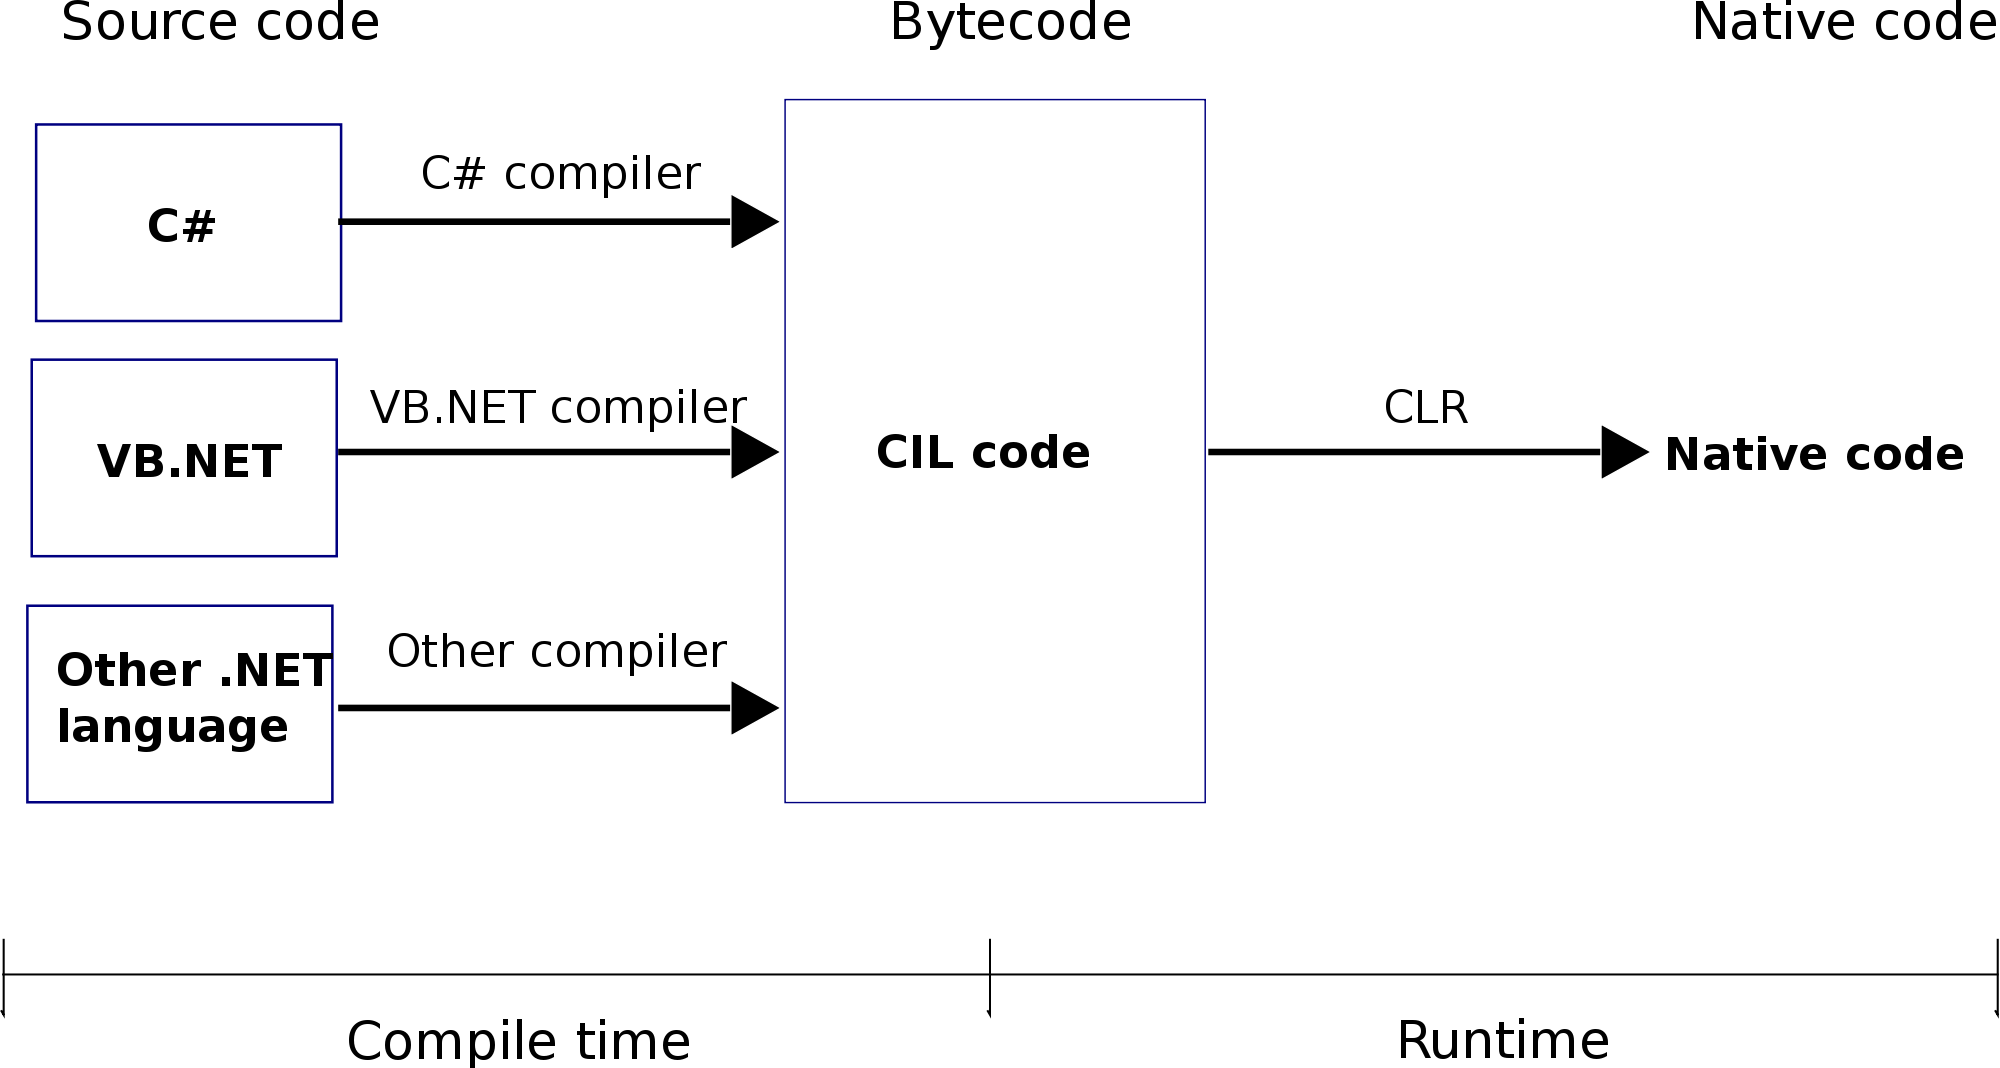
\includegraphics[width=1\textwidth]{graphics/CLR.png}
    \\
    \only{\tiny{Wikipedia \\ \url{http://tr.im/pWUi}}}
  \end{column}
  \end{columns}
\end{frame}
%Briefly, VMs emulate an operating system, or computer hardware. We'll be talking about a specific kind of VM, the process VM, that acts as a runtime environment for a program.

\begin{frame}
  \frametitle{High-level vs Bytecode}
  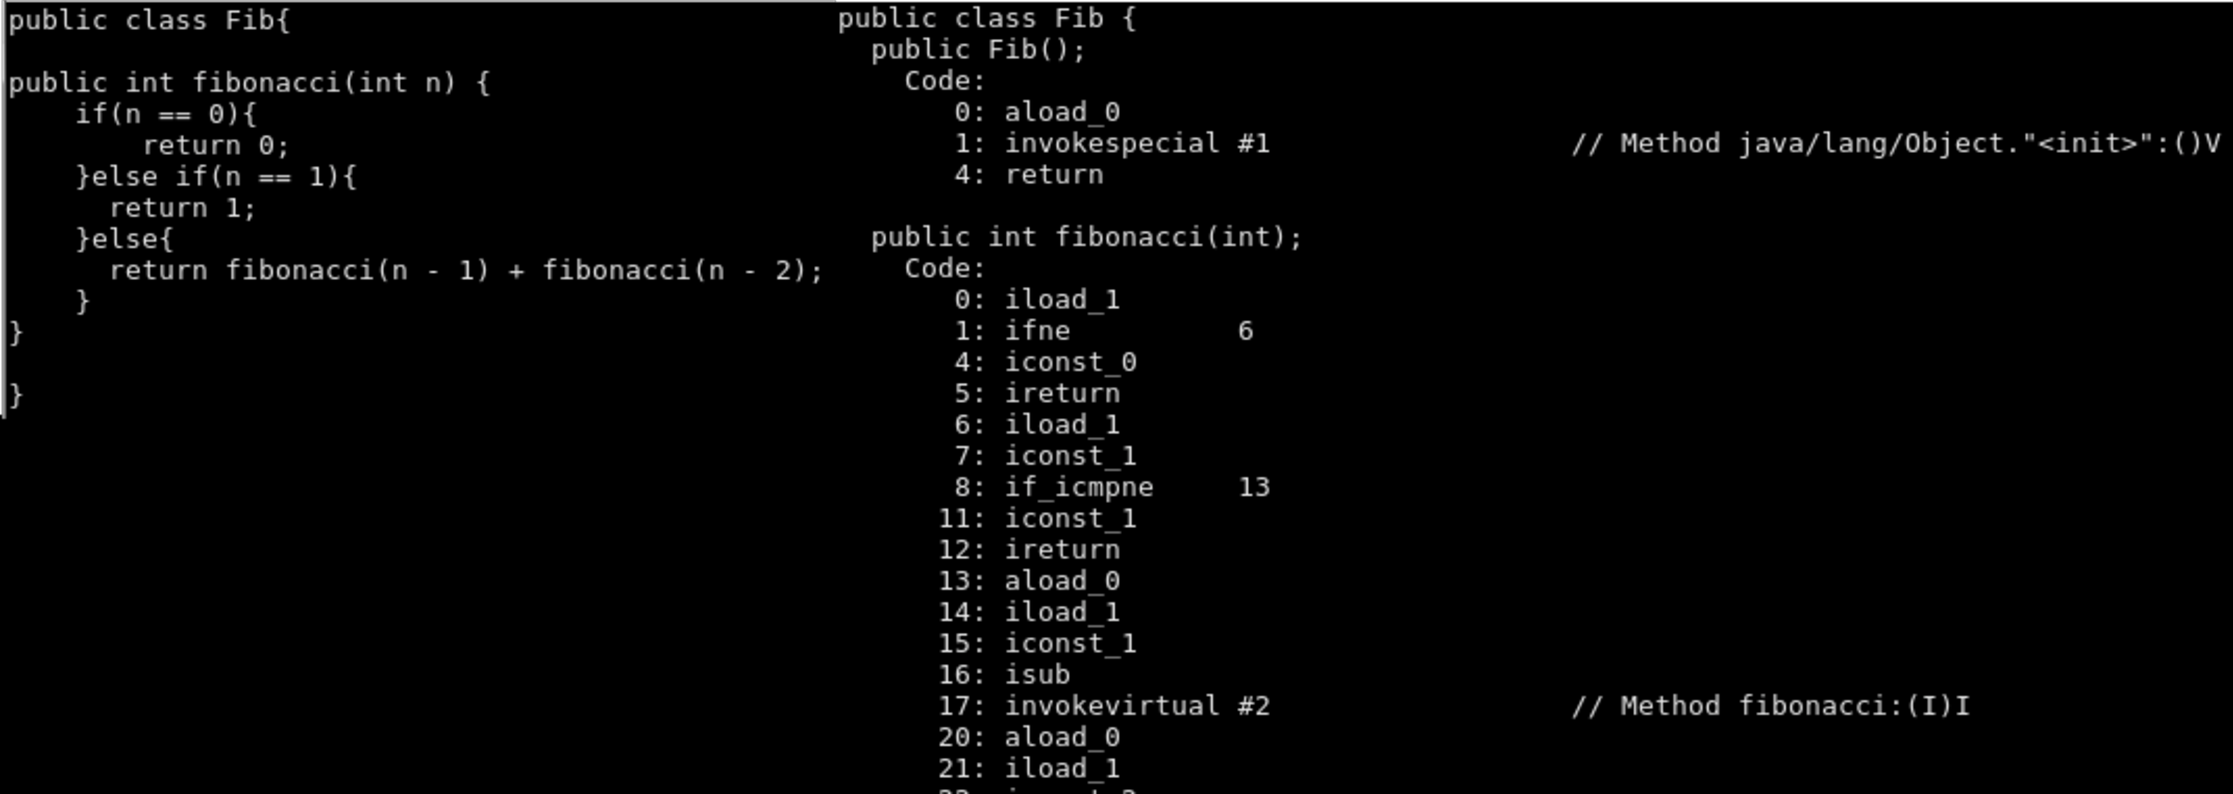
\includegraphics[width=1.5\textwidth]{graphics/FibCompair.pdf}
\end{frame}

\subsection{Markup Languages}

\begin{frame}
  \frametitle{Markup Languages}
  
  \begin{columns}
  \begin{column}{0.6\textwidth}
  \begin{itemize}
  	\item 
	\item 
	\item 
	\item 
	\item 
  \end{itemize}
  \end{column}
  \end{columns}
\end{frame}

\section[Difficulty]{What makes Interop difficult?}

\begin{frame}
  \frametitle{Some common difficulties in interop}
  
  \begin{columns}
  \begin{column}{0.6\textwidth}
  \begin{itemize}
  	\item 
	\item 
	\item 
	\item 
	\item 
  \end{itemize}
  \end{column}
  \end{columns}
\end{frame}

\section[Handling interop]{Concepts in overcoming difficulties}

\subsection{Metadata}

\begin{frame}
  \frametitle{Metadata and type conversion}

	Metadata: Data about data
	
	{\tt (def mylist [1, 2, 3, 4])}
	
	{\tt (with-meta mylist \{:length 4, :type Integer\})}
	\linespace
	In Clojure:
	\begin{itemize}
	\item lists are untyped; can contain entries of different types.
	\item metadata, added as above, is all user-controlled.
	\end{itemize}
\end{frame}

\begin{frame}
    \frametitle{Why Metadata?}
  \begin{columns}
  \begin{column}{0.6\textwidth}

    \begin{itemize}   
    \item Decontextualized data can carry context with it
    \item Data transfer between languages with different type strictness.
    \end{itemize}
  \end{column}
   %add example here...
  \begin{column}{0.6\textwidth}
  
  \end{column}
  
  \end{columns}
\end{frame}

\subsection{Standards}

\begin{frame}
  \frametitle{The importance of Standards}
  
  \begin{columns}
  \begin{column}{0.6\textwidth}
  \begin{itemize}
  	\item 
	\item 
	\item 
	\item 
	\item 
  \end{itemize}
  \end{column}
  \end{columns}
\end{frame}

\section[Conclusions]{Conclusions}

\begin{frame}
  \frametitle{Conclusions}
  
  \begin{columns}
  \begin{column}{0.6\textwidth}
  \begin{itemize}
  	\item 
	\item 
	\item 
	\item 
	\item 
  \end{itemize}
  \end{column}
  \end{columns}
\end{frame}




\begin{frame}
	\frametitle{The End!}
	
	
		
	\linespace
	\linespace
	
	Contact:  
	\begin{itemize}
		\item \texttt{malone153@morris.umn.edu}
	\end{itemize}
	
	\linespace
	\linespace
	
	\begin{center}
	{\huge Questions?}
	\end{center}
\end{frame}

\section*{References}

\begin{frame} 
	\frametitle{References} 
	
	\bibliography{bibliography}
	
	\linespace
	\begin{center}
	See the GECCO '09 paper for additional references.
	\end{center}
\end{frame} 

\end{document}


